\NeedsTeXFormat{LaTeX2e}
\documentclass[a4paper,12pt,
headsepline,        % Linie Kopfzeile / Text
oneside,            % einseitig
bibtotoc,           % Lit.verz. ins Inh.verz.
pointlessnumbers,   % kein Punkt nach letzter Gliederungsziffer
%DIV=15,              % Satzspiegel auf 15er Raster, schmalere Ränder   
BCOR15mm             % mehr li. Rand zum Binden der Arbeit
%,draft
]{scrbook}
\KOMAoptions{DIV=last}

\pagestyle{headings}
\usepackage{blindtext}

% für Texte in deutscher Sprache
\usepackage[ngerman]{babel}
\usepackage[utf8]{inputenc}
\usepackage[T1]{fontenc}
\usepackage{tikz}

\usepackage{algpseudocode}
\usetikzlibrary{decorations.pathreplacing}

% Helvetica als Standard-Dokumentschrift
\usepackage[scaled]{helvet}
\renewcommand{\familydefault}{\sfdefault} 

\usepackage{graphicx}

% Tabellen mit fester Gesamtbreite und variabler Spaltenbreite
\usepackage{tabularx} 
%\begin{tabularx}{Breite}    {Spaltendefinition} ... \end{tabularx}
%\begin{tabularx}{\textwidth}{XXl} ...               \end{tabularx}

\usepackage{url}              % \url{http://...} in Schreibmaschinenschrift
\usepackage{color}            % zum Setzen farbigen Textes
\usepackage{amssymb, amsmath} % Pakete für Mathe-Umgebungen und -Symbole


\usepackage{setspace} % Paket für div. Abstände, z.B. ZA
\setlength{\parindent}{0pt}
\setlength{\parskip}{1.4ex plus 0.35ex minus 0.3ex}

% Tiefe, bis zu der Überschriften in das Inhaltsverzeichnis kommen
\setcounter{tocdepth}{3} % ist Standard

% Beispiele für Quellcode
\usepackage{listings}
\lstset{language=Java,
  showstringspaces=false,
  frame=single,
  numbers=left,
  basicstyle=\ttfamily,
  numberstyle=\tiny}

% hier Namen etc. einsetzen
% TODO hier anpassen
\newcommand{\fullname}{Florian Krötz}
\newcommand{\email}{florian.kroetz@uni-ulm.de}
\newcommand{\titel}{Cache-optimierte QR-Zerlegung}
\newcommand{\jahr}{2018}
\newcommand{\matnr}{884948}
\newcommand{\gutachterA}{Dr.~Michael Lehn}
\newcommand{\gutachterB}{Dr.~Andreas Borchert}
\newcommand{\betreuer}{Dr.~Michael Lehn}

% hier die Fakultät auswählen
%\newcommand{\fakultaet}{---  Im Quellcode anpassen nicht vergessen! ---}
%\newcommand{\fakultaet}{Ingenieurwissenschaften, Informatik und Psychologie}
\newcommand{\fakultaet}{Mathematik und\\Wirtschafts-\\wissenschaften}
%\newcommand{\fakultaet}{Medizin}
%\newcommand{\fakultaet}{Naturwissenschaften}

% hier das Institut einsetzen
\newcommand{\institut}{Institut für Numerische Mathematik}

%color in tables
\usepackage{colortbl}
\definecolor{Gray}{rgb}{0.80784, 0.86667, 0.90196} %dunkelblau
\definecolor{Lightgray}{rgb}{0.9176, 0.95, 0.95686} %hellblau
\definecolor{Akzent}{rgb}{0.6627, 0.63529, 0.55294} %akzentfarbe
\setlength{\arrayrulewidth}{0.1pt}


\pdfinfo{
  /Author (\fullname)
  /Title (\titel)
  /Producer     (pdfeTex 3.14159-1.30.6-2.2)
  /Keywords ()
}

\usepackage{hyperref}
\hypersetup{
pdftitle=\titel,
pdfauthor=\fullname,
pdfsubject={Diplomarbeit},
pdfproducer={pdfeTex 3.14159-1.30.6-2.2},
colorlinks=false,
pdfborder=0 0 0	% keine Box um die Links!
}

%Trennungsregeln
\hyphenation{Sil-ben-trenn-ung}

\begin{document}
\frontmatter

% Titelseite
\thispagestyle{empty}
\begin{addmargin*}[4mm]{-10mm}


\includegraphics[height=1.8cm]{images/unilogo_bild}
\hfill

\includegraphics[height=1.8cm]{images/unilogo_wort}\\[1em]

{\footnotesize
%{\bfseries Universität Ulm} \textbar ~89069 Ulm \textbar ~Germany
\hspace*{115mm}\parbox[t]{35mm}{\bfseries Fakultät für\\
\fakultaet\\

\mdseries \institut}\\[2cm]

\parbox{120mm}{\bfseries \LARGE \titel}\\[2.5em]
{\footnotesize Bachelorarbeit an der Universität Ulm}\\[3em]

{\footnotesize \bfseries Vorgelegt von:}\\
{\footnotesize \fullname\\\email}\\[2em]
{\footnotesize \bfseries Gutachter:}\\                     
{\footnotesize\gutachterA\\
\gutachterB}\\[2em]
{\footnotesize \bfseries Betreuer:}\\ 
{\footnotesize\betreuer}\\\\
{\footnotesize\jahr}
}
\end{addmargin*}


% Impressum
\clearpage
\thispagestyle{empty}
{ \small
  \flushleft
  Fassung \today \\\vfill
  \copyright~\jahr~\fullname\\[0.5em]
% Wenn Sie Ihre Arbeit unter einer freien Lizenz bereitstellen möchten, können Sie die nächste Zeile in Ihren Code aufnehmen. Bitte beachten Sie, dass Sie hierfür an allen Inhalten, inklusive enthaltener Abbildungen, die notwendigen Rechte benötigen! Beim Veröffentlichungsexemplar Ihrer Dissertation achten Sie bitte darauf, dass der Lizenztext nicht den Angaben in den Metadaten der genutzten Publikationsplattform widerspricht. Nähere Information zu den Creative Commons Lizenzen erhalten Sie hier: https://creativecommons.org/licenses/
%This work is licensed under the Creative Commons Attribution 4.0 International (CC BY 4.0) License. To view a copy of this license, visit \href{https://creativecommons.org/licenses/by/4.0/}{https://creativecommons.org/licenses/by/4.0/} or send a letter to Creative Commons, 543 Howard Street, 5th Floor, San Francisco, California, 94105, USA. \\
  Satz: PDF-\LaTeXe
}


% ab hier Zeilenabstand etwas größer 
\setstretch{1.1}

%\onehalfspacing % nur dann, wenn gefordert; ist sehr groß!!

\tableofcontents

\mainmatter
% TODO Kapitel einbinden
\chapter{Einleitung}
%Ziel dieser Bachelorarbeit ist es die QR-Zerlegung zu beschreiben. 
Als QR-Zerlegung bezeichnet man die Zerlegung der Matrix $A$ in eine  orthogonale Matrix $Q$ und eine obere Dreiecksmatrix $R$.
\begin{align*}
	A = Q \cdot R
\end{align*} 

In dieser Arbeit wird die Berechnung der QR-Zerlegung mittels Householder-Transformation betrachtet. 

Neben der Householder-Transformation kann die QR-Zerlegung auch mittels Givens-Rotationen oder mit dem Gram-Schmidtschen Orthogonalisierungsverfahrens berechnet werden.

Die QR-Zerlegung bietet folgende Möglichkeiten:
%Mit eine QR-Zerlegung kann man:
\begin{itemize}
	\item Gleichungssysteme mit schlechter Kondition lassen sich mittels QR-Zerlegung stabiler als mit dem Gausschen Eliminationsverfahren (LR-Zerlegung) lösen. 

	\item Lösen von linearen Ausgleichsproblemen durch die Methode der kleinsten Fehlerquadrate. 
	
%	\item Im QR-Verfahren ist die QR-Zerlegung eine Kernoperation, weil in jedem Iterationsschritt eine QR-Zerlegung berechnet wird.	Das QR-Verfahren berechnet die Eigenwerte einer Matrix.	
	
	\item Berechnung von Eigenwerten einer Matrix mittels QR-Verfahren. Im QR-Verfahren ist die QR-Zerlegung eine Kernoperation, da in jedem Iterationsschritt eine QR-Zerlegung berechnet wird.
\end{itemize}

%Weil die QR-Zerlegung bei diesen Problemen oft verwendet wird, empfiehlt es sich, die Berechnung der OR-Zerlegung zu optimieren.

Weil die QR-Zerlegung bei den aufgezählten Problemen häufig verwendet wird, empfiehlt es sich, die Berechnung der OR-Zerlegung zu optimieren.

Um die Prozessorkapazität optimal zu nutzen, ist es sinnvoll, die QR-Zerlegung mit einem cache-optimierten Algorithmus zu berechnen.
Dadurch ist es möglich, die angegebene Maximalleistung des Prozessors zu erreichen.

\subsubsection{Cache-Optimierung}
Der Cache ist ein schneller Datenspeicher. Daten, die vom Prozessor verarbeitet werden sollen, müssen immer zuerst in den Cache geladen werden.
Der Zugriff auf Daten, die im RAM liegen, dauert sehr viel länger als der Zugriff auf Daten, die im Cache liegen.
Aus diesem Grund ist es sinnvoll, die Algorithmen so zu gestalten, dass eine optimale Übertragung erfolgt.

Ziele der Cache-Optimierung:
\begin{itemize}
	\item Mehrfaches Laden von Daten soll vermeiden werden.
	\item Die Daten müssen in der Reihenfolge, in der sie verwendet werden, im RAM liegen.
	\item Sequentiell im RAM liegende Daten werden durch Prefetching effizient in den Cache geladen.
\end{itemize}

Prefetching ist die Eigenschaft des Prozessors, Zugriffsmuster auf den Speicher zu erkennen und vorherzusagen.	

\subsubsection{Intel MKL}
Die Intel MKL (Math Kernel Library) \cite{mkl} ist eine Bibliothek der Firma Intel, in welcher mathematische Funktionen enthalten sind.
%Die Intel MKL ist eine Bibliothek der Firma Intel. Die Abkürzung MKL steht für Math Kernel Library.
%In der Bibliothek sind mathematische Funktionen enthalten.
Die MKL implementiert diese Funktionen sehr effizient, damit der Prozessor die angegebene theoretische Maximalleistung erreichen kann.

%Die MKL beinhaltet BLAS-Routinen (Basic Linear Algebra Subprogramms) und LAPACK-Routinen (Linear Algebra Package) \cite{DGEQR2}.

%Es sind Funktionen der linearen Algebra wie BLAS (Basic Linear Algebra Subprogramms) und LAPACK (Linear Algebra Package) implementiert.

In der MKL sind die beiden Programmbibliotheken BLAS (Basic Linear Algebra Subprogramms) und LAPACK (Linear Algebra Package) implementiert. 
Diese Funktionen aus der Teilmenge der linearen Algebra sind für die Berechnung der QR-Zerlegung elementar erforderlich.

BLAS enthält grundlegende und LAPACK weiterentwickelte Funktionen der linearen Algebra.










\chapter{BLAS}
Die Abkürzung BLAS steht für Basic Linear Algebra Subprograms. 
BLAS-Bibliotheken enthalten elementare Operationen der linearen Algebra.


\section{Datenstruktur für Matrizen}
Vollbesetzte Matrizen werden bei BLAS entweder zeilen- oder spaltenweise abgespeichert. Das bedeutet, dass entweder die Zeilen- oder die Spalten der Matrix hintereinander im Speicher stehen.  

\begin{align*}
	A=
	\left(\begin{array}{ccc}
	a_{1,1} & a_{1,2} & a_{1,3} \\ 
	a_{2,1} & a_{2,2} & a_{2,3} \\ 
	a_{3,1} & a_{3,2} & a_{3,3} 
	\end{array} \right) \in \mathbb{R}^{m \times n}
\end{align*}
Matrix $A$ Zeilenweise gespeichert\\
\begin{tikzpicture}
	\draw[semithick] (0,0) -- (9,0);
	\draw[semithick] (0,1) -- (9,1);
	\draw[semithick] (0,0) -- (0,1);
	\draw[semithick] (1,0) -- (1,1);
	\draw[semithick] (2,0) -- (2,1);
	\draw[semithick] (3,0) -- (3,1);
	\draw[semithick] (4,0) -- (4,1);
	\draw[semithick] (5,0) -- (5,1);
	\draw[semithick] (6,0) -- (6,1);
	\draw[semithick] (7,0) -- (7,1);
	\draw[semithick] (8,0) -- (8,1);
	\draw[semithick] (9,0) -- (9,1);
	
	\draw (0.5,0.5) node {$a_{1,1}$};
	\draw (1.5,0.5) node {$a_{1,2}$};
	\draw (2.5,0.5) node {$a_{1,3}$};
	\draw (3.5,0.5) node {$a_{2,1}$};
	\draw (4.5,0.5) node {$a_{2,2}$};
	\draw (5.5,0.5) node {$a_{2,3}$};
	\draw (6.5,0.5) node {$a_{3,1}$};
	\draw (7.5,0.5) node {$a_{3,2}$};
	\draw (8.5,0.5) node {$a_{3,3}$};
	
	\draw[->,line width=0.4mm] (0,-.5) -- (0,0);
	\draw (0,-0.8) node {*data};
	\draw[->,line width=0.4mm] (0,-.25) -- (3,-.25);
	\draw (3,-0.8) node {incRow};
\end{tikzpicture}\\
Matrix $A$ Spaltenweise gespeichert\\
\begin{tikzpicture}
\draw[semithick] (0,0) -- (9,0);
\draw[semithick] (0,1) -- (9,1);
\draw[semithick] (0,0) -- (0,1);
\draw[semithick] (1,0) -- (1,1);
\draw[semithick] (2,0) -- (2,1);
\draw[semithick] (3,0) -- (3,1);
\draw[semithick] (4,0) -- (4,1);
\draw[semithick] (5,0) -- (5,1);
\draw[semithick] (6,0) -- (6,1);
\draw[semithick] (7,0) -- (7,1);
\draw[semithick] (8,0) -- (8,1);
\draw[semithick] (9,0) -- (9,1);

\draw (0.5,0.5) node {$a_{1,1}$};
\draw (1.5,0.5) node {$a_{2,1}$};
\draw (2.5,0.5) node {$a_{3,1}$};
\draw (3.5,0.5) node {$a_{1,2}$};
\draw (4.5,0.5) node {$a_{2,2}$};
\draw (5.5,0.5) node {$a_{3,2}$};
\draw (6.5,0.5) node {$a_{1,3}$};
\draw (7.5,0.5) node {$a_{2,3}$};
\draw (8.5,0.5) node {$a_{3,3}$};
	
\draw[->,line width=0.4mm] (0,-.5) -- (0,0);
\draw (0,-0.8) node {*data};
\draw[->,line width=0.4mm] (0,-.25) -- (3,-.25);
\draw (3,-0.8) node {incCol};
\end{tikzpicture}\\


Eine Datenstruktur benötigt folgende Elemente:
\begin{itemize}
	\item einen Zeiger auf eine Speicherfläche
	\item Informationen ob die Matrix zeilen- oder spaltenweise gespeichert ist 
	\item die Dimension der Matrix.
\end{itemize}


Eine derartige Datenstruktur könnte in C/C++ so aussehen.
\begin{lstlisting}
struct Matrix {
  double * data;
  std::ptrdiff_t incRow, incCol;
  std::size_t numRows, numCols;
}
\end{lstlisting}

Diese Datenstruktur ist für Matrixeinträge vom Type double.

Die Variablen für die Speicherverwaltung(Zeile 3) sind vom Typ ptrdiff\_t und die Variablen für die Dimensions Informationen sind Vom Typ size\_t.

ptrdiff\_t und size\_t sind Datentypen für Ganzzahlen. Der Unterschied zwischen den Datentypen ist size\_t kann nur Werte Darstellen die größer gleich 0 sind, ptrdiff\_t dann auch negative Werte Darstellen.

Die das incRow und incCol aus negative Werte haben könne ist Sinnvoll, wenn man zugriff auf Einen Matrix Block haben will in anderer Reihenfolge.

Für Intel MKL Routinen müssen die Matrizen zeilenweise gespeichert sein.
Das bedeutet incCol ist gleich 1.

\subsubsection{Beispiel}
Angenommen es wurde genügend Speicher für eine Matrix $A$ allociert und die Werte 1 bis 25 liegen hintereinander im Speicher.
Dann lässt sich die Matrix
\begin{align*}
	A = \begin{pmatrix}
	 1 &  2 &  3 &  4 &  5 \\
	 6 &  7 &  8 &  9 & 10 \\
	11 & 12 & 13 & 14 & 15 \\
	16 & 17 & 18 & 19 & 20 \\
	21 & 22 & 23 & 24 & 25 
	\end{pmatrix}
\end{align*}
durch die folgende Datenstruktur repräsentieren.
\begin{lstlisting}
struct Matrix A;
A.data = /*pointer to data*/;
A.numRows = 5; 
A.numCols = 5;
A.incRow = A.numCols;
A.incCol = 1;
\end{lstlisting}
Die Matrix 
\begin{align*}
B = \begin{pmatrix}
25 &  20 &  15 & 10 \\
24 &  19 &  14 & 9 \\
23 &  18 &  13 & 8 
\end{pmatrix}
\end{align*}
lässt sich mit folgender Datenstruktur repräsentieren.
\begin{lstlisting}
struct Matrix B;
B.data = A.data[4*A.incRow + 4*A.incCol];
B.numRows = 3; 
B.numCols = 4;
B.incRow = -A.incCol;
B.incCol = -A.incRow;
\end{lstlisting}
Diese Datenstruktur nutzt für die Daten den selben Speicherbereich wie die Matrix $A$. 

Der data-Pointer wurde auf das letzte Element der Matrix $A$ gesetzt.

Blablabla incRow Trans blabla


\newpage
\section{Einige BLAS-Routinen}
Im Folgenden werden einige BLAS-Routinen beschrieben, die bei der QR-Zerlegung benutzt werden.
BLAS-Routinen werden nach folgendem Schema benannt:
Der erste Buchstabe im Namen gibt an für welchen Datentype die Funktion implementiert wurde. Der Rest beschreibt die Funktion der Funktion.\\
Beispiel \glqq dgemm\grqq{}: Das \glqq d\grqq{} zeigt, dass die Funktion ist für Doubles gilt und  \glqq gemm\grqq{} steht für \glqq generel Matrix Matrix\grqq{}. Die  Funktion berechnet also das Matrix-Matrix Produkt für Matrizen, deren Einträge Doubles sind.

\subsection{Matrix-Matrix Produkt (gemm)}
Die Funktion \glqq gemm\grqq{} berechnet das Matrix-Matrix Produkt.
Der Funktion werden die Matrizen $A$, $B$ und $C$ und die Skalare $\alpha$ und $\beta$ übergeben. Außerdem werden 2 Flags übergeben ob die Matrizen $A$ und $B$ transponiert werden sollen.\\
Die Funktion berechnet
\begin{align}
	C \leftarrow \beta  C + \alpha  A  B
\end{align}
Falls $\beta = 0$ wird die Matrix $C$ zuerst mit Nullen initialisiert. Falls $C$ Einträge hat die NaN (Not a Number) sind, werden diese somit mit 0 überschrieben.

%%TODO
\cite{blast}
Blas tecnicla forum netlib
%%http://www.netlib.org/blas/blast-forum/

\subsection{Matrix-Vektor Produkt (gemv)}
Die Funktion \glqq gemv\grqq{} berechnet das Matrix-Vektor Produkt.
Der Funktion werden die Matrix $A$, die Vektoren $x$ und $y$, und die Skalare $\alpha$ und $\beta$ übergeben. Außerdem wird ein Flag übergeben, das anzeigt ob die Matrix $A$ transponiert werden soll.\\
Die Funktion berechnet
\begin{align}
y \leftarrow \beta  y + \alpha A x 
\end{align}
Falls $\beta = 0$ wird der Vektor $y$ zuerst mit Nullen initialisiert. Falls $y$ Einträge hat, die NaN (Not a Number) sind, werden diese mit 0 überschrieben.

\subsection{Rank1 update (ger)}
Die Funktion \glqq ger\grqq{}  berechnet ein dyadisches Produkt aus den Vektoren $x$ und $y$, skaliert die daraus resultierende Matrix mit $\alpha$ und addiert das Ergebnis auf $A$.\\
Der Funktion werden die Matrix $A$, die Vektoren $x$ und $y$ und das Skalar $\alpha$ übergeben.\\
Die Funktion berechnet
\begin{align}
A \leftarrow A + \alpha  x y^T
\end{align}

\subsection{Matrix-Matrix Produkt (trmm)} \label{fkt:trmm}
Die Funktion \glqq trmm\grqq{} berechnet das Matrix-Matrix Produkt einer Dreiecksmatrix mit einer voll besetzten Matrix.
Der Funktion wird die Dreiecksmatrix $A$, die Matrix $B$ und das Skalar $\alpha$ übergeben. Außerdem werden Flags mit übergeben, die anzeigen ob $A$ eine obere oder untere Dreiecksmatrix ist, ob $A$ eine strikte oder unipotente Dreiecksmatrix ist, ob $A$ von links oder rechts auf $B$ multipliziert werden soll und ob $A$ transponiert werden soll. Diese Eigenschaften werden unten in $op(\cdot)$ zusammengefasst. \\
Die Funktion berechnet
\begin{align}
B \leftarrow  \alpha \cdot op(A) \cdot B \qquad \text{oder} \qquad B \leftarrow  \alpha \cdot B \cdot op(A)
\end{align}
\subsection{Matrix-Vektor Produkt (trmv)} \label{fkt:trmv}
Die Funktion \glqq trmv\grqq{} berechnet das Matrix-Vektor Produkt für Dreiecksmatrizen.
Die Funktion berechnet
\begin{align}
x \leftarrow \alpha  Ax %\qquad \text{or} \qquad x \leftarrow \alpha * A^T*x
\end{align}


Dreiecksmatrizen die von den Funktionen \glqq trmm\grqq{} und \glqq trmv\grqq{} verarbeitet werden sind quadratische Matrizen von denen nur der obere oder unter Dreiecks teil betrachtet wird.
Das heißt die Matrix liegt als Quadratische Matrix im Speicher. Die Funktion beachtet nur die Einträge über oder unter der Diagonalen.
Wird dem Algorithmus mit einem Flag angezeigt das es sich um eine eine unipotente Dreiecksmatrix handeln soll, werden die Diagonaleinträge im Speicher nicht beachtet sondern vom Algorithmus als 1 angenommen. \cite{blast}



\chapter{QR-Zerlegung}

\section{Definition}
Eine Matrix $A \in \mathbb{R}^{m \times n}$ , $m \ge n$ besitzt eine eindeutige QR-Zerlegung.
\begin{align}
	A = QR
\end{align}
mit einer orthogonalen Matrix $ Q \in \mathbb{R}^{m \times m} $ und einer oberen Dreiecksmatrix $ R \in \mathbb{R}^{n \times n}$ \cite{num1}

Eine QR Zerlegung kann mit einer Householder-Transformation berechnet werden.

\subsection{Beispiel}
Lösung eines Minimierungsproblem
\begin{align}
	\min_{x \in \mathbb{R}^n} \|Ax-b\|^2 \label{eq1}
\end{align}
mit Matrix $A \in \mathbb{R}^{m\times n}$ mit $rang(A) = n < m$ für die eine QR Zerlegung existiert.
$R$ besitzt die Gestalt 
\begin{align*}
	R=	
	\left(\begin{array}{ccc}
		*&*&* \\ 
		&*&* \\ 
		& &* \\ \hline
		& 0 &
	\end{array} \right)
	=
	\left(\begin{array}{c}
	 \\ 
	\hat{R} \\ 
	 \\ \hline
	0
	\end{array} \right) 
\end{align*}

$\hat{R}$ stellt eine obere Dreiecksmatrix dar.
Damit kann man das Minimierungs Problem wie folgt modifizieren mit $A=QR$
\begin{align}
		\min_{x \in \mathbb{R}^n} \|Ax-b\|^2 =
		\min_{x \in \mathbb{R}^n} \|Q^T(Ax-b)\|^2 =
		\min_{x \in \mathbb{R}^n} \|Rx-Q^Tb\|^2
\end{align}
Also löst
\begin{align}
Rx=Q^Tb \label{solvminqr}
\end{align}
das Minimierungsproblem (\ref{eq1}). Da $R$ eine Dreiecksmatrix ist, lässt sich (\ref{solvminqr}) leicht mit Rückwärtseinsetzen  lösen.

\section{Householder-Transformation}
%Ein Vektor  $v \in \mathbb{R}^n$ dann wird die $n \times n$ Matrix 
Eine Matrix $H \in \mathbb{R}^{n \times n}$ 
\begin{align}
	H = I - 2 \dfrac{vv^T}{v^Tv} \label{eq:HHM}
\end{align}
wird als Householder-Transformation und der Vektor $v \in \mathbb{R}^n$ als Householder-Vektor bezeichnet.
Eine Householder-Transformation $H = I - 2 \dfrac{vv^T}{v^Tv}$ ist orthogonal und symmetrisch. \cite{num1}\\
Die Householder-Transformation spiegelt den Vektor $x$ auf die Achse $x_1$.
Dazu multipliziert man $H$ von links auf $x$
\begin{align}
	Hx=\alpha e_1 \label{eq:spiegelung}
\end{align}
mit dem Skalar $\alpha \in \mathbb{R}$ und $e_1$ als ersten kanonischen Einheitsvektor. Der Householder-Vektor steht senkrecht auf der Ebene an welcher $x$ gespiegelt wird.\\
Die Abbildung \ref{fig:HHolder} veranschaulicht die Spiegelung des Vektors $x$ an der gestrichelt eingezeichneten Ebene auf die Achse $x_1$.
\begin{figure}[H]
	\centering
	\begin{tikzpicture}

\draw[->] (-2,0) -- (3,0);
\draw[->] (0,-1) -- (0,3);

\draw[->,line width=0.5mm] (0,0) -- (-1,2);
\draw[->,line width=0.5mm] (0,0) -- (2.24,0);

\draw[dashed] (-0.44,-0.9) -- (1.34,2.68);
%\draw[->,line width=0.5mm] (0,0) -- (-0.9, 0.44);
%\draw[->,line width=0.5mm] (0,0) -- (-1,0.61);
\draw[->,line width=0.5mm] (0,0) -- (1,-0.61);





\filldraw[red, opacity=0.5] (0,0)--(-0.1467,-0.3000) arc (240:330:.3339) -- (0,0) ;
\draw[black, opacity=1] (0,0)--(-0.1467,-0.3000) arc (240:330:.3339) -- (0,0) ;
\filldraw(0.03,-0.2) circle (.02cm) ;

%Beschriftung
\draw (3.4,-0.1) node {$x_1$};
\draw (-0.1,3.3) node {$x_2$};

\draw (.45, -.6) node {$v$};
\draw (-.25, 1) node {$x$};
\draw (1,0.3) node {$Hx$};


\end{tikzpicture}
	\caption{Beispiel Householder-Transformation mit $x=(-1,2)^T$}
	\label{fig:HHolder}
\end{figure}




\subsection{Householder Vector}
Damit (\ref{eq:spiegelung}) gilt, wird der Vektor folgendermaßen berechnet. 
In dem man (\ref{eq:HHM}) in (\ref{eq:spiegelung}) einsetzt
\begin{align*}
	Hx &= x - 2\dfrac{vv^T}{v^Tv} x = x - \underbrace{2\dfrac{v^Tx}{v^Tv}}_{\lambda} v = x - \lambda v \overset{!}{=} \alpha e_1 \\
	&\Longrightarrow v \in \text{span}\{x - \alpha e_1\}
\end{align*}
erhält man dass $v$ in dem Span $x  - \alpha e_1$ liegt.\cite{num1}
%Mit $Hx = x - 2\dfrac{vv^T}{v^Tv} x = x - \lambda v \overset{!}{=} \alpha e_1$ folgt $v \in \text{span}\{x - \alpha e_1\}$. \cite{num1}\\

Setzt man $v = t(x - \alpha e_1)$ in $Hx = \alpha e_1 $(\ref{eq:spiegelung}) ein, erhält man 
\begin{align*}
	Hx =& x - \dfrac{2}{v^Tv}v(v^Tx) = x - 2\dfrac{v^Tx}{v^Tv}v\\
	=& x - 2\dfrac{ t(x - \alpha e_1)^Tx}{ t(x - \alpha e_1)^T t(x - \alpha e_1)} t(x - \alpha e_1)
	= x - 2\dfrac{ (x - \alpha e_1)^Tx}{ (x - \alpha e_1)^T (x - \alpha e_1)} (x - \alpha e_1)
	\\
	=& x - \dfrac{(x - \alpha e_1)^Tx}{\|x - \alpha e_1\|_2^2} (x - \alpha e_1)
	=\underbrace{\left(1 - \dfrac{2(x - \alpha e_1)^Tx}{\|x - \alpha e_1\|_2^2}\right)}_{ \overset{!}{=} 0 } x + \alpha e_1 \underbrace{\dfrac{2(x - \alpha e_1)^Tx}{\|x - \alpha e_1\|_2^2} }_{\overset{!}{=} 1} \overset{!}{=} \alpha e_1
\end{align*}

Damit das Letzte $=$ gilt muss gelten.
\begin{align*}
	1 &= \dfrac{2(x - \alpha e_1)^Tx}{\|x - \alpha e_1\|^2}\\
	\Leftrightarrow (x - \alpha e_1)^T(x - \alpha e_1) &= 2 x^T x - 2\alpha x_1 \\
	\Leftrightarrow x^Tx -2\alpha x_1 + \alpha^2 &= 2 x^T x - 2\alpha x_1\\
	\Leftrightarrow \alpha &= \pm \sqrt{x^Tx}
\end{align*}

Das Vorzeichen von  $\alpha = \pm \sqrt{x^Tx}$ kann man frei wählen, um $ v = x - \alpha e_1$ zu berechnen.

Wählt man das Vorzeichen positiv kann Auslöschung auftreten, falls $x$ annähernd ein positives Vielfaches von $e_1$ ist.

LAPACK \cite{DGEQR2} vermeidet die Auslöschung indem das Vorzeichen entgegengesetzt gewählt wird. Das bedeutet $x$ wird immer auf die gegenüberliegende Seite gespiegelt.

Im Skript von Numerik 1 \cite{num1} wird das Vorzeichen immer positiv gewählt\\ $\alpha = |\sqrt{x^Tx}| = \|x\|_2$. Eine mögliche Auslöschung im Fall $ x_1 > 0$ wird hier durch die folgende Umformung vermieden.
\begin{align*}
	v_1 = x_1 - \|x\|_2 = \dfrac{x_1^2 - \|x\|_2^2}{x_1 + \|x\|_2}
	=\dfrac{-(x_2^2+...+x_n^2)}{x_1 + \|x\|_2}
\end{align*}

%Der Vorteil bei der von LAPACK verwendeten Methode ist, dass hier nur die Norm berechnet werden muss, wohingegen bei dem anderen Algorithmus das Skalarprodukt $x^Tx$ berechnet werden muss. Dies kann bei Vektoren mit vielen Einträgen und großen Werten zu einem Überlauf führen. Es muss jedoch ein Algorithmus gewählt werden, der die Norm berechnet $\|x\|=\sqrt{x^Tx}$ ohne das Skalarprodukt explizit auszurechnen.

Um den Vektor $v$ später auf der frei werdenden Diagonalen von $A$ speichern zu können wird er auf $v_1 = 1$ normiert. Dies geschieht mit 
\begin{align}
	v = \dfrac{x - \alpha e_1}{x_1 - \alpha}
	\label{eq:calcV}
\end{align}

Mit der Normierung kann man den Faktor $\tau = \dfrac{2}{v^Tv}$ berechnen. Setze dazu (\ref{eq:calcV}) in die Definition von $\tau$ ein.
\begin{align*}
	\tau = \dfrac{2}{v^Tv} = \dfrac{2 (x_1 - \alpha)^2}{(x - \alpha e_1)^T (x - \alpha e_1)} = \dfrac{2 (x_1 - \alpha)^2}{\|x\|^2_2 - 2\alpha x^Te_1 + \alpha^2} =  \dfrac{2 (x_1 - \alpha)^2}{ 2\alpha (\alpha - x_1)} = \dfrac{x_1 - \alpha}{\alpha}
\end{align*}

Mit dem Faktor $\tau = \dfrac{2}{v^Tv}$ kann man die Householder-Transformation schreiben als
\begin{align*}
	H = I - 2 \dfrac{vv^T}{v^Tv} = I - \tau v v^T
\end{align*}



\begin{algorithm}
	\caption{Housholder-Vector(LAPACK DLARFG)}
	\begin{algorithmic}
		\State Input: $x \in \mathbb{R}^n$ 
		\State $\alpha = -1 * \text{sign}(x_1) \|x\|_2$
		\State $\tau = \dfrac{x_1 - \alpha}{\alpha}$
		\State $v=\dfrac{x - \alpha e_1}{x_1 - \alpha}$
		\State Output: Householder-Vektor $v$, $\tau$
	\end{algorithmic} 
	\label{alg:unblockedqr}
\end{algorithm}


\subsection{Householder-Transformation anwenden}
Ein aufwändiges Matrix-Matrix-Produkt kann bei der Anwendung einer Housholder-Transformation $H = I - \tau vv^T$ auf die Matrix $A$ umgangen werden, indem man geschickt klammert.
\begin{align*} 
H A =(I - \tau vv^T) A= A - \tau (vv^T )A = A - \tau v(v^TA)
\end{align*}
Statt eines Matrix-Matrix-Produkts muss man nur ein Matrix-Vektor-Produkt und ein dyadisches Produkt berechnen.
%Das Matrix-Vektor-Produkt und das dyadische Produkt haben nur einen Aufwand von $O(n^2)$.

\subsection{QR-Zerlegung mittels Housholder-Transformationen}
Um $A$ in eine obere Dreiecksmatrix $R$ zu transformieren, wird eine Folge von Housholder-Transformationen auf $A$ angewendet.

Zuerst wird aus der ersten Spalte der Matrix $A$ ein Householder-Vektor berechnet, dann wird die  Householder-Transformationen auf die Matrix angewandt.
Diese Housholder-Transformation erzeugt Nullen in der ersten Spalte unterhalb es ersten Eintrags.
Damit eine obere Dreiecksmatrix entsteht, wird als nächstes die Matrix $A$ ohne die erste Zeile und Spalte betrachtet. Aus der ersten Spalte der neu betrachteten Matrix wird wieder ein Householder-Vektor berechnet und die Householder-Transformationen auf die Matrix angewandt.
Fährt man nach diesem Schema immer weiter fort entsteht eine ober Dreiecksmatrix.
%Mit Householder-Transformationen kann eine Matrix $A$ wie folgt transformieren.
\begin{align*}
	H_1 A= \left( 
	\begin{array}{cccc}
	* & * & * & * \\ 
	0 & * & * & * \\ 
	0 & * & * & * \\ 
	0 & * & * & *
	\end{array}
	\right)
	\quad , \quad
	H_2 H_1 A= \left( 
	\begin{array}{cccc}
	* & * & * & * \\ 
	0 & * & * & * \\ 
	0 & 0 & * & * \\ 
	0 & 0 & * & *
	\end{array}
	\right)
\end{align*} 


%\begin{align*}
%	H_i = \begin{pmatrix}
%	I_{i-1} & 0\\
%	0 & \tilde{H_i}
%	\end{pmatrix}
%\end{align*}
%$I_{i-1}$ bezeichnet die $i-1$ dimensionale Einheitsmatrix, $\tilde{H_i}$ ist eine Householder-Transformation.



So erhält man die Faktorisierung
\begin{align*}
R = H_{n-1} H_{n-2}\cdot ...\cdot H_1 A \Leftrightarrow A = (H_1\cdot ...\cdot H_{n-1})R \Rightarrow Q = H_1\cdot ... \cdot H_{n-1}
\end{align*}
$Q$ ist das Produkt aller Householder-Transformationen.
Diese Vorgehensweise führt zum Algorithmus \ref{alg:unblockedqr}. 
\begin{algorithm}[H]
	\caption{Ungeblockte Housholder-Transformation}
	\begin{algorithmic}
	\State Input: $A \in \mathbb{R}^{m \times n}$
	\For {i = 0,1,2,..., n}
		\State ($v_i$, $\tau_i$) $\leftarrow$ householdervector($A(i:m,i)$)
		\State $w \leftarrow v^T*A(i:m,i:n)$ (dgemv)
		\State $ A(i:m,i:n) \leftarrow \tau * v * w + A $ (dger)
		\If {i > m}
			\State $A(i + 1 : m, i) \leftarrow v(2 : m - i + 1)$
		\EndIf
	\EndFor	
	\State Output: $A$ QR zerlegt, Vektor $\tau \in \mathbb{R}^n$
\end{algorithmic} 
\label{alg:unblockedqr}
\end{algorithm}

Matizen sind 0 indizeiert notiert

Dieser Algorithmus \ref{alg:unblockedqr} überschreibt die Matrix $A$ mit $R$.
Aufgrund der Dreiecksstruktur von $R$,
können unter der Diagonale die Housholder-Vektoren gespeichert werden. 
Die Householder-Vektoren haben die Form 
\begin{align*}
v^{(j)} = ( \underbrace{0,...,0}_{j-1},1,	v_{j+1}^{(j)},...,v_{m}^{(j)}  )
\end{align*}
Da die ersten $j-1$ Einträge Null sind und der Vektor so normiert wurde das der $j$ Eintrag gleich 1 ist, müssen die ersten $j$ Einträge nicht gespeichert werden.
Die Householder-Vektoren können somit unterhalb der Diagonalen gespeichert werden.
Die Matrix $A$ hat somit die Form
\begin{align*}
	A = 
	\left(\begin{array}{ccc}
	r_{1,1}   &  r_{1,2}  & r_{1,3} \\ 
	v_2^{(1)} &  r_{2,2}  & r_{2,3} \\ 
	v_3^{(1)} & v_3^{(2)} & r_{3,3} \\ 
	v_4^{(1)} & v_4^{(2)} & v_4^{(3)}
	\end{array} \right) 
\end{align*}


\section{Geblockte QR-Zerlegung}
Ein geblockter Algorithmus ist sinnvoll, um bei großen Matrizen den Cache optimal zu nutzen.

Im folgenden wird ein geblockter Algorithmus beschrieben wie er auf von LAPACK verwendet wird. Die entsprechende Funktion bei LAPACK heißt \glqq DGEQRF\grqq{} \cite{DGEQRF}.

Die Idee beim geblockten Algorithmus ist die Matrix in Blöcke aufzuteilen, die geblockte QR-Zerlegung für die Blöcke zu berechnen und die dabei verwendeten Householder-Transformationen auf den Rest der Matrix anzuwenden.


Betrachte dazu die Matrix $A \in \mathbb{R}^{m \times n}$ geblockt, mit einer geeigneten Blockgröße $bs$.
\begin{align}
	A = \left(\begin{array}{l|l}
	A_{0, 0} & A_{0, \text{bs}} \\ \hline
	A_{\text{bs}, 0}   & A_{\text{bs}, \text{bs}} 	
	\end{array} \right) \label{equ:blockA}
\end{align}
Die Abbildung \ref{fig:blockA} zeigt schematisch die Partitionierung von A.

Die Blockgröße $bs$ wird so gewählt das die Geschwindigkeit der ungeblockten QR-Zerlegung für den Block $ \left(\dfrac{A_{0, 0}}{A_{\text{bs}, 0}} \right)$ optimal ist.

Für diesen Block wird nun die  QR-Zerlegung mit dem ungeblockten Algorithmus (Algorithmus \ref{alg:unblockedqr}) berechnet.
\begin{align}
	\left(\begin{array}{l} 
	A_{0, 0} \\ \hline
	A_{\text{bs}, 0}
	\end{array}\right)
	\leftarrow
	\left(\begin{array}{l} 
	Q_{0, 0}  \backslash R_{0,0} \\ \hline
	Q_{\text{bs}, 0} 
	\end{array}\right)
\end{align}

Im Block $A_{0, 0}$ steht nun auf und über der Diagonalen $R_{0,0}$. Unterhalb der Diagonalen und im Block $A_{\text{bs}, 0}$ stehen die Householder-Vektoren.

Nun muss man die bei der ungeblocketn QR-Zerlegung verwendeten Housholder-Transformationen auf die Restliche Matrix $ \left(\dfrac{A_{0, \text{bs}}}{A_{\text{bs}, \text{bs}}} \right)$ anwenden.



Man kann das Produkt mehrerer Householder-Transformationen schreiben als
\begin{align*}
H_1H_2...H_k = I - VTV^T \qquad \text{mit}\qquad H_i = I - \tau_i v_iv_i^T
\end{align*} \cite{Joffrain:2006:AHT:1141885.1141886}

Die Anwendung der Matrix $I - V*T*V^T$ auf $\left(\dfrac{A_{\text{bs}, \text{bs}}}{A_{\text{bs}, \text{bs}}} \right)$ erfolgt in 2 Schritten.

Zuerst wird von der Funktion \glqq larft \grqq{}  die Matrix $T$ berechnet.
Dann wird $I - V*T*V^T$ von der Funktion \glqq larfb\grqq{} auf $\left(\dfrac{A_{\text{bs}, \text{bs}}}{A_{\text{bs}, \text{bs}}} \right)$ angewendet.


\begin{align}
	\left(\begin{array}{l} 
	A_{0, \text{bs}} \\ \hline
	A_{bs, \text{bs}}
	\end{array}\right)
	\leftarrow
	H^T \left(\begin{array}{l} 
	A_{0, \text{bs}} \\ \hline
	A_{bs, \text{bs}}
	\end{array}\right)
\end{align}

%Betrachte nun den Block $A_{bs, \text{bs}}$ wie in (\ref{equ:blockA}), in der Abbildung \ref{fig:blockA} gestrichelt Dargestellt.

Der Block $A_{bs, \text{bs}}$ wird erneut aufgeteilt. Das ist in Abbildung \ref{fig:blockA} gestrichelt dargestellt.

Fahre solange fort bis $A_{bs, \text{bs}}$ gleich der Blockgröße ist.
\begin{figure}[H]
	\centering
	\begin{tikzpicture}
\draw[semithick] (0,0) -- (4,0) -- (4,4) -- (0,4) -- (0,0);

\draw[semithick] (1,0) -- (1,4);
\draw[semithick] (0,3) -- (4,3);
\draw[semithick,opacity=0.3] (0,4) -- (1,3);

\draw[dashed,opacity=0.5] (2,0) -- (2,3);
\draw[dashed,opacity=0.5] (1,2) -- (4,2);
\draw[dashed,opacity=0.5] (1,3) -- (2,2);


\draw (0.5,3.5) node {$A_{0,0}$};
\draw (0.5,1.5) node {$A_{bs,0}$};
\draw (2.5,3.5) node {$A_{0,bs}$};
\draw (2.5,1.5) node {$A_{bs,bs}$};
\draw[decorate, decoration={brace,mirror}, yshift=-.2ex]  (0,0) -- node[below=0.4ex] {$bs$}  (1,0);
\draw[decorate, decoration={brace}, xshift=-.2ex]  (0,3) -- node[left=0.4ex] {$bs$}  (0,4);
\draw[decorate, decoration={brace,mirror}, yshift=-3ex]  (0,0) -- node[below=0.4ex] {$n$}  (4,0);
\draw[decorate, decoration={brace}, xshift=-3.5ex]  (0,0) -- node[left=0.4ex] {$m$}  (0,4);

\end{tikzpicture}
	\caption{Partitionierung vom A}
	\label{fig:blockA}
\end{figure}

\subsection{Berechnung der Matrix $T$}
Die Funktion \glqq larft\grqq{} berechnet die Matrix $T$. 

Sie bekommt eine Dreiecksmatrix $V \in \mathbb{R}^{m \times k}$ einen Vektor $\tau \in \mathbb{R}^k$ und eine Matrix $T\in \mathbb{R}^{k\times k}$ übergeben. 

In der Dreiecksmatrix $V$ stehen die Householder-Vektoren,
im Vektor $\tau$ die zu den Householder-Vektoren gehörende $\tau_i$.

Die Funktion berechnet eine obere Dreiecksmatrix $T$ so dass
\begin{align*}
	H_1H_2...H_k = I - VTV^T \qquad \text{mit}\qquad H_i = I - \tau_i v_iv_i^T
\end{align*}

Warum und wie das Funktoniert wird hier beschreiben \cite{Joffrain:2006:AHT:1141885.1141886}.




\subsection{Anwenden von $I - VTV^T$ larfb}

Die Funktion \glqq larfb \grqq{} wendet die Matrix $I - VTV^T$ auf eine Matrix $C$ an.

Sie bekommt eine untere Dreiecksmatrix $V \in \mathbb{R}^{m \times k}$, eine obere Dreiecksmatrix $T \in \mathbb{R}^{k \times k}$ und eine Matrix $C \in \mathbb{R}^{m \times n }$ übergeben.

In der Dreiecksmatrix $V$ stehen die Householder-Vektoren,
im Vektor $\tau$ die zu den Householder-Vektoren gehörende $\tau_i$.
Die Matrix $C$ wird upgedatet indem die  Block Reflector Matrix $ 	H = C - V T V^T $ von rechts auf die Matrix $ C $ angewendet wird. 

Ein weiterer Übergabeparameter gibt an ob die Block Reflector Matrix transponiert werden soll.
Die Funktion berechnet also
\begin{align*}
	C \leftarrow H C = C - V T V^T C \quad \text{oder} \quad 	C \leftarrow H^T C = C - V T^T V^T C
\end{align*}

Der Zweck der Funktion ist es die Householder-Transformationen, die bei der Bereicherung der QR-Zerlegung für einen Block entstanden sind, auf die restliche Matrix anzuwenden.
Die Abbildung \ref{fig:patrA} zeigt wie die Matrix $A$ für die Funktion Partitioniert wird.
\begin{figure} [H]
	\centering
	\begin{tikzpicture}
\draw[semithick] (0,0) -- (4,0) -- (4,4)-- (0,4)-- (0,0);


\draw[semithick] (1,0) -- (1,4);
\draw[semithick] (0,3) -- (4,3);
\draw[line width=0.5mm] (0,4) -- (0,0) -- (1,0) -- (1,3) -- (0,4);


\draw[decorate, decoration={brace,mirror}, yshift=-.2ex]  (0,0) -- node[below=0.4ex] {$k$}  (1,0);
\draw[decorate, decoration={brace}, xshift=-.2ex]  (0,3) -- node[left=0.4ex] {$k$}  (0,4);
\draw[decorate, decoration={brace,mirror}, yshift=-3ex]  (0,0) -- node[below=0.4ex] {$n$}  (4,0);
\draw[decorate, decoration={brace}, xshift=-3ex]  (0,0) -- node[left=0.4ex] {$m$}  (0,4);

\draw (0.3,3.3) node {$v_1$};
\draw (0.5,1.5) node {$v_2$};
\draw (2.5,3.5) node {$c_1$};
\draw (2.5,1.5) node {$c_2$};



\end{tikzpicture}
	\caption{Partitionierung vom A für larfb}
	\label{fig:patrA}
\end{figure}
Falls $m > k $ werden die Matrizen $V$ und $C$ aufgeteilt in $V=\left(\dfrac{V_1}{V_2}\right)$ und $C=\left(\dfrac{C_1}{C_2}\right)$.
%Sodass $V_1 \in \mathbb{R}^{k \times k}$ und $C \in \mathbb{R}^{k \times n}$
Dabei wird $V$ genau so geteilt, dass $V_1 \in \mathbb{R}^{k\times k}$ der quadratisch Dreiecksteil der Matrix ist und $V_2 \in \mathbb{R}^{m-k\times k}$ der Rest der Matrix. Die Matrix $C$ wird in $C_1 \in \mathbb{R}^{k \times n}$ und $C_2 \in \mathbb{R}^{m-k \times n}$  aufgeteilt. Die Aufteilung ist so gewählt das das Matrix-Matrix-Produkt $V_1 \cdot C_1$ und $V_2 \cdot C_2$ möglich ist.\\
Diese Aufteilung ist notwendig da die BLAS-Funktion trmm (matrix-matrix product where one input matrix is triangular) nur für Quadratische Dreiecksmatrizen implementiert ist.

Im Fall $ m = k $ ist die Aufteilung nicht notwendig da $ V $ quadratisch ist.




\begin{align*}
	C \leftarrow  C - \underbrace{V T V^T C}\\
	V \cdot T \cdot V^T \cdot C\\ 
	(C^T \cdot V \cdot T^T \cdot V^T)^T 
\end{align*}



Dies führt zu den
\begin{algorithm}[H]
	\caption{Block reflector anwenden}
	\label{alg:applyblockref}
	\begin{algorithmic}
		\State 	$W \leftarrow C_1^T$ (copy)
		\State	$W \leftarrow W * V_1 $ (trmm)
		\If {m > k}
			\State $W \leftarrow W + C_2^T*V_2$ (gemm)
		\EndIf
		\State 	$ W \leftarrow W * T^T \quad \text{or}\quad  W * T$ (trmm)
		\If {m > k}
			\State $C_2 \leftarrow C_2 - V_2 * W^T$ (gemm)
		\EndIf
		\State 	$ W \leftarrow W * V_1^T $ (trmm)
		\State 	$ C_1 \leftarrow C_1 - W^T $
	\end{algorithmic}
\end{algorithm}





\subsection{Iterativer Algorithmus}
\begin{algorithm}[H]
	\caption{Iterativer Algorithmus}
	\label{alg::italg}
	\begin{algorithmic}
		\For {i = 0 : n}
			\State QR = A;
			\If {i + ib > n}
				\State Calc T: $H=I-VTV^T$
				\State Apply H: $A=H^TA$
			\EndIf
		\EndFor
	\end{algorithmic}
\end{algorithm}

\chapter{Implementierung und Benchmarks}
Die verwendete Bibliothek wurde in der Vorlesung High Performance Computing 1 entwickelt \cite{HPC1}.

Die Bibliothek ist in C++ geschrieben. Es sind Klassen für Matrizen und Vektoren implementiert, sowie einige BLAS-Routinen.

Die Matrix-Klassen erlauben den zugriff auf Matrixblöcke. 
\begin{lstlisting}
GenerelMatrix<T> A(5,5);
print(A);
print(A.block(2,2));
print(A.block(2,2).view(Trans::view));
\end{lstlisting}



Beispiel Ungeblockte QR Implementierung vom Algorithmus \ref{alg:unblockedqr}
\begin{lstlisting}
size_t mn = std::min(m,n);
DenseVector<T> work(mn);
for (std::size_t i = 0; i < mn; ++i){
  householderVector(A(i,i), A.col(i+1,i),tau(i));
  if (i < n && tau(i) != 0) {
    AII = A(i,i);
    A(i,i) = 1;
    mv(1, A.block(i,i+1).view(hpc::matvec::Trans::view),
       A.col(i,i), 0, work.block(i+1));
    rank1(-tau(i), A.col(i,i), work.block(i+1), 
          A.block(i,i+1));
    A(i,i) = AII;
  }
}
\end{lstlisting}

Die anderen Algorithem wurden analog Implementiert siehe Anhang.


\section{Aufwand}

Die QR-Zerlegung einer Matrix $A \in \mathbb{R}^{m \times n}$  erfordert
\begin{align*}
	n^2(m-\frac{1}{3} n) + {\cal O}(mn)
\end{align*}
Rechenoperationen. Quelle???

\subsection{FLOPS}
FLPOS (Floating Point Operations Per Second) 

\section{Fehlerschätzer}

Um zu testen ob die QR-Zerlegung korrekt ist, ist ein Fehlerschätzer notwendig.
Es wurde der Fehlerschätzer von ATLAS\cite{atlas} verwendet.
\begin{align}
	err = \dfrac{\|A - QR\|_i}{\|A\|_i \cdot \min(m,n) \cdot \varepsilon}
\end{align}
$\|\cdot\|_i$ ist eine passende Norm.
Die Matrizen $Q$ und $R$ sind die QR-Zerlegung der Matrix $A \in \mathbb{R}^{m \times n}$.
$\varepsilon$ ist die kleinste darstellbare Zahl.\\
Die QR-Zerlegung ist gut genug falls der Fehler kleiner 1 ist $ err < 1 $.

Als Norm wurde die Zeilensummennorm $\|\cdot\|_\infty$ gewählt.
Diese ist für eine Matrix $A \in \mathbb{R}^{m\times n}$ gegeben durch
\begin{align*}
	\|A\|_\infty = \max_{i=1,...,m} \sum_{j=1}^{n} |a_{ij}|
\end{align*}

Diese Norm wurde gewählt das sie sich leicht berechnen lässt.

$\epsilon$ ist auf dem Test-System $2.220446\cdot10^{-16}$


\section{Benchmarks}

\subsection{Test System}

Getestet wurde auf einem System mit einer Intel(R) Core(TM) i5-3470 CPU mit 3.20GHz. 

Die Theoretische peak performance errechnet sich aus der Taktrate mal die Registerbreite mal 2. Quelle???


Die CPU des Test Systems hat eine Taktrate von 3.20GHz.
Die AVX-Register sind 256-Bit groß. Darin haben 4 double Platz.

\begin{align*}
	\text{Taktrate} \cdot \text{Registerbreite} \cdot 2= 3,20 \text{ GHz} \cdot 4 \cdot 2 = 25,6 \text{ GFLOPs}
\end{align*}

\begin{figure}[H]
	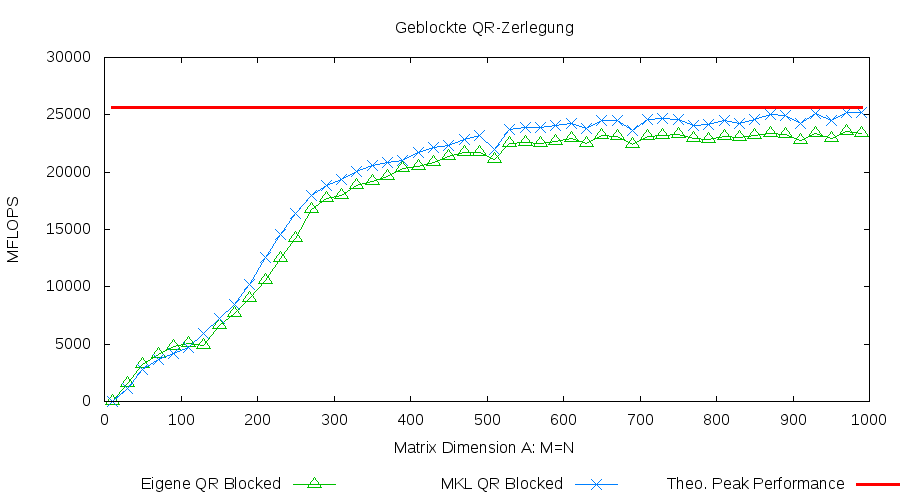
\includegraphics[width=\textwidth]{images/blk.png}
	\caption{Benchmark geblockte QR-Zerlegung}
	\label{img:blk}
\end{figure}

\begin{figure}[H]
	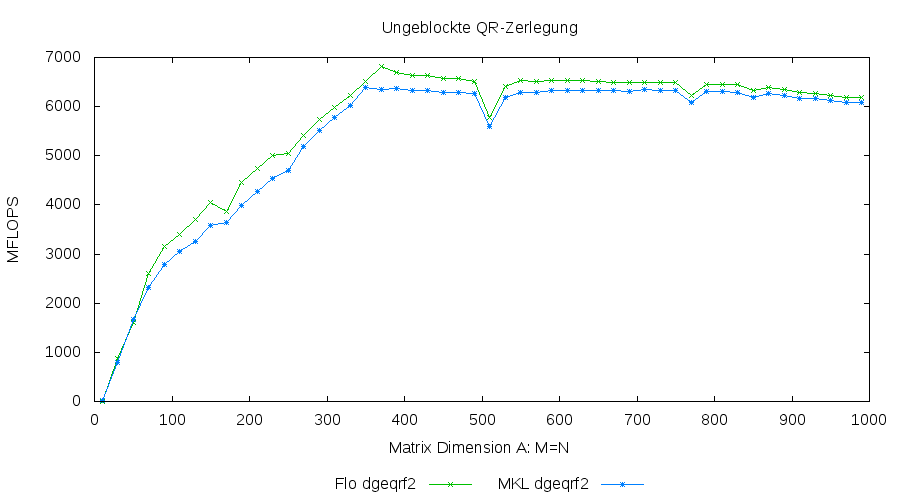
\includegraphics[width=\textwidth]{images/unblk.png}
	\caption{Benchmark ungeblockte QR-Zerlegung}
	\label{img:unblk}
\end{figure}

Dreiecke und Sternchen









	 



\appendix
% TODO Anhänge einbinden
\chapter{Quelltexte}

In diesem Anhang sind einige wichtige Quelltexte aufgeführt.

\begin{lstlisting}
#include<stdio.h>
int main(int argc, char ** argv) {
  printf("Hallo HPC \n");
  return 0;
}
\end{lstlisting}


\backmatter

\bibliographystyle{plaindin} % Nummern und alphabetisch sortiert
%\bibliographystyle{alphadin} % Buchstaben und sortiert
%\bibliographystyle{abbrvdin} % Nummern und abgekürzte Namen
%\bibliographystyle{unsrtdin} % Nummern und unsortiert
%\bibliographystyle{lit}
\bibliography{bibliography.bib}


\clearpage
\thispagestyle{empty}

Name: \fullname \hfill Matrikelnummer: \matnr \vspace{2cm}

\minisec{Erklärung}

Ich erkläre, dass ich die Arbeit selbständig verfasst und keine anderen als die angegebenen Quellen und Hilfsmittel verwendet habe.\vspace{2cm}

Ulm, den \dotfill

\hspace{10cm} {\footnotesize \fullname}
\end{document}
